\documentclass[final,t]{beamer}
\mode<presentation>
{
%  \usetheme{Warsaw}
%  \usetheme{Aachen}
%  \usetheme{Oldi6}
%  \usetheme{I6td}
  \usetheme{I6dv}
%  \usetheme{I6pd}
%  \usetheme{I6pd2}
}
% additional settings
\setbeamerfont{itemize}{size=\normalsize}
\setbeamerfont{itemize/enumerate body}{size=\normalsize}
\setbeamerfont{itemize/enumerate subbody}{size=\normalsize}
\newcommand{\danielsize}{\fontsize{90}{85}\selectfont}
\newcommand{\davidsize}{\fontsize{88}{85}\selectfont}
\newcommand{\mikesize}{\fontsize{84}{85}\selectfont}

% additional packages
\usepackage{times}
\usepackage{amsmath,amsthm, amssymb, latexsym}
\usepackage{exscale}
\usepackage{multirow}
%\boldmath
\usepackage{booktabs, array}
%\usepackage{rotating} %sideways environment
\usepackage[english]{babel}
\usepackage[latin1]{inputenc}
\usepackage[orientation=landscape,size=custom,width=300,height=200,scale=2.6]{beamerposter}
\listfiles
\graphicspath{{figures/}}
% Display a grid to help align images
%\beamertemplategridbackground[1cm]

\title{\huge Unsupervised Automatic Spike Sorting} 
\author{\danielsize{Daniel Sommerman}, \davidsize{David Brody}, \mikesize{Michael Gummelt}}
\institute[Stanford University]{Department of Computer Science,
  Stanford University, Stanford, California}
\date[Dec. 14 , 2011]{Dec. 14 , 2011}

% abbreviations
\usepackage{xspace}
\makeatletter
\DeclareRobustCommand\onedot{\futurelet\@let@token\@onedot}
\def\@onedot{\ifx\@let@token.\else.\null\fi\xspace}
\def\eg{{e.g}\onedot} \def\Eg{{E.g}\onedot}
\def\ie{{i.e}\onedot} \def\Ie{{I.e}\onedot}
\def\cf{{c.f}\onedot} \def\Cf{{C.f}\onedot}
\def\etc{{etc}\onedot}
\def\vs{{vs}\onedot}
\def\wrt{w.r.t\onedot}
\def\dof{d.o.f\onedot}
\def\etal{{et al}\onedot}
\makeatother

\newcommand{\comment}[1]{}

%%%%%%%%%%%%%%%%%%%%%%%%%%%%%%%%%%%%%%%%%%%%%%%%%%%%%%%%%%%%%%%%%%%%%%%%%%%%%%%%%%%%%%%%%%%%%%%%%%%%%%%%%%%%
%%%%%%%%%%%%%%%%%%%%%%%%%%%%%%%%%%%%%%%%%%%%%%%%%%%%%%%%%%%%%%%%%%%%%%%%%%%%%%%%%%%%%%%%%%%%%%%%%%%%%%%%%%%%
\begin{document}
\begin{frame}{} 
  \begin{columns}[t]
    \begin{column}{.3\linewidth}

      %%%%%%%%%%%%%%%%%%%%%%%%%%%%%%%%%%%%%%%%%%%%%%%%%%%%%%%%%%%%%%%%%%%%%%%%%%%%%%%%%%%%%%%%%%%%%%%%%%%%%%%%%%%%

      \begin{block}{Introduction}
        Extracellular neurophysicological data recorded from a
        microelectrode is a mixture of the responses from the many
        surrounding cells. The responses are then clustered into
        similar shaped groups which represent different cells. Our
        project aims to take this analysis step which is usually done
        manually and automate it using machine learning.
      \end{block}

      %%%%%%%%%%%%%%%%%%%%%%%%%%%%%%%%%%%%%%%%%%%%%%%%%%%%%%%%%%%%%%%%%%%%%%%%%%%%%%%%%%%%%%%%%%%%%%%%%%%%%%%%%%%%

       \begin{block}{Problem and Data Description }
        We are given extracellular recordings from 60 different
        channels. Each channel represents a data stream of voltage
        potentials at a specific microelectrode. A sample recording
        looks like the following:
        \vskip1em
         \begin{center}
           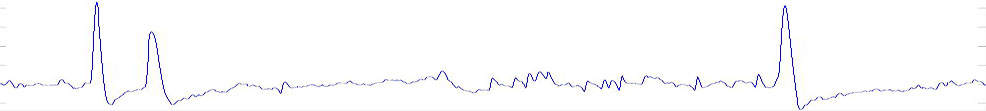
\includegraphics[width=0.8\linewidth]{images/voltagetrace_2_small.jpg}
         \end{center}
         \vskip1em
         The aim of the project is to cluster each spike into clusters
         which each share a similar shape.  Example cluster centers
         could look like the following:
         \vskip1em
         \begin{table}[ht]
           \centering
           \begin{tabular}{c c c }
             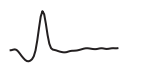
\includegraphics[width=0.2\linewidth]{images/WaveShape1.png} &
             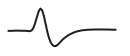
\includegraphics[width=0.2\linewidth]{images/WaveShape2.png} &
             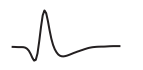
\includegraphics[width=0.2\linewidth]{images/WaveShape3.png}
           \end{tabular}
         \end{table}
         \begin{center}
         \end{center}
         \vskip1em
       \end{block}
       
       \begin{block}{Model Definitions}
          \noindent{\textbf{Model Parameters}}\par
          N = # of datapoints per channel \break
          CH = # of channels \break
          S = # of points to smooth raw data over \break
          T = Threshold for spikes \break
          L = # points to take from left of spike location
          R = # points to take from right of spike location
          \vskip1em
          \noindent{\textbf{Definitions}}\par
          We begin with the raw waveform: \break
          \begin{center}
          $R = {{R^i \in R^N; i = 1,...,CH}}$ \break
          \end{center}
          Smoothing over S points we define a new waveform where $R^i_j$
          is the jth datapoint in the ith channel: \break
          \begin{center}
          $W^i_j = \frac{1}{s}\sum_{s=-S/2}^{S/2}R^{i}_{j+s}$ \break
          \end{center}
          \break
          We then define $W'$ as the zero mean normalized to the standard
          deviation on each channel of $W$. The next step is to
          separate out the possible spikes to cluster. We define the
          spike locations of interest as:
          \break
          \begin{center}
          $P = \{ i; \frac{\partial}{\partial W} = 0 \cap 
          (W_1'(P_i) > T \cup ... \cup W_{CH}'(P_i) > T) \cap i \in
          1,...,N \} $ \break
          \end{center}
          \break
          Peaks are then cut to ensure that they are a minimum of
          $\alpha = 15$ from each other. To form a single feature vector $X^{(i)}$ we take the
          surrounding points on each channel and concatentate them. \break
          \begin{center}
          $X^{(i)}_j = W'^{floor(i/(L+R+1))+1}_{mod(j, L+R+1) + P(i)}
          ; i = 1,...,|P|, j = 1,...,(L+R+1)*CH$ \break
          \end{center}
          \break
          X is the feature vector we use to then cluster on.
       \end{block}

      %%%%%%%%%%%%%%%%%%%%%%%%%%%%%%%%%%%%%%%%%%%%%%%%%%%%%%%%%%%%%%%%%%%%%%%%%%%%%%%%%%%%%%%%%%%%%%%%%%%%%%%%%%%%
      

      %%%%%%%%%%%%%%%%%%%%%%%%%%%%%%%%%%%%%%%%%%%%%%%%%%%%%%%%%%%%%%%%%%%%%%%%%%%%%%%%%%%%%%%%%%%%%%%%%%%%%%%%%%%%

    \end{column}
    \begin{column}{.3\linewidth}
      



      \begin{block}{Pipeline}
        \begin{center}
          \includegraphics[width=0.8\linewidth,height=15cm]{images/noexist.png}
        \end{center}
        
        We paramaterize our feature vectors from the raw data with the following representations:
        \begin{center}
          $X = M(R; S,T,L,R)$ 
        \end{center}
        \break
        We then use different methods to reduce the dimensionality of
        the feature vectors to improve performance and to emphasize
        more discrimanent features.
        \break
        \begin{center}
        $Red(X,N,M; X \in \mathbb{R}^N) = Y \in \mathbb{R}^M$ 
        \break
        \end{center}
        Clustering then takes the dimension reduced feature vectors
        and assigns them to clusters which represent possible cells.
        
     \end{block}
     
     \begin{block}{Dimensionality Reduction}
       \noindent{\textbf{Principle Component Analysis}}\par
       
At this point, we have our features and are ready to run unsupervised
learning algorithms on the data set. However, as we began experimenting
with our data set, we realized that the time needed to learn on our data
set was simply too great. We needed a way to reduce the dimensionality of
our features. Since a feature vector consists of 30 measurements for 60
channels each, we have features in $\mathbb{R}^{1800}$.

The first approach we took was to apply PCA and take the top 300 principal
components and project our features into that space, $\mathbb{R}^{300}$.
Performing this optimization allowed us to run k-means clustering in
roughly 13\% of the time without compression. We experimented with
projecting into different dimension subspaces and found 300 to be a good
dimension that saves enough on running time without sacrificing too much
in terms of underfitting.

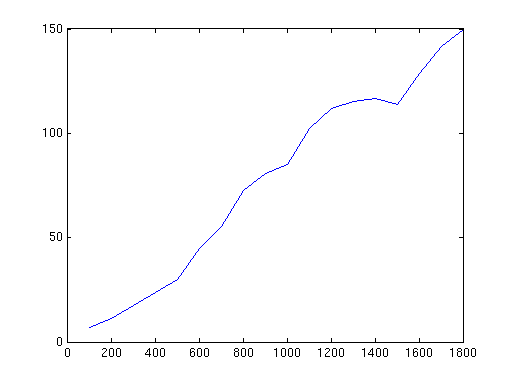
\includegraphics[width=0.8\linewidth,height=40cm]{images/dim_vs_runningtime.png}
       
In this plot of time taken to run kmeans verses dimensionality of the
feature, we can clearly see how we save considerable time by reducing the
dimension of the problem. PCA was a huge win in being able to rapidly
prototype our clustering algorithms.

       \noindent{\textbf{Polynomial Fitting}}\par
         We also tried fitting polynomials of various degrees. In this
         case, we let our feature vector be in $\mathbb{R}^{60(n+1)}$,
         representing the coefficients to 60 polynomials (one for each
         channel), each of degree $n$.

         We didn't have time to gather metrics on using this form of
         dimensionality reduction, but we are confident that this could be
         a good way to model a channel's response, since each channel
         outputs smooth data that could fit a reasonably low degree
         polynomial well.
     \end{block}
   \end{column}
   
    %%%%%%%%%%%%%%%%%%%%%%%%%%%%%%%
    
    \begin{column}{.3\linewidth}
      \begin{block}{Clustering}
        \noindent{\textbf{G-Means}}\par
        One way to choose k in the k-means algorithm is to use an algorithm
developed in 2003 by Greg Hamerly and Charles Elka, presented in the NIPS
2003 conference. In this method, a small value for k is
chosen and kmeans is run. For each cluster produced, we use a
heuristic function to decide whether to split that cluster: the
Anderson-Darling statistic. If that statistic is greater than
some threshold critical value, then we decide that the cluster should be
split. The Anderson-Darling statistic is computed as follows:
$$
A^2(Z) = -n - \frac{1}{n}\sum_{i=1}^n (2i -
1)[\log(z_i)+\log(1-z_{n+1-i})]
$$$$
A^2_*(Z) = A^2(Z)(1 + 4/n - 25/n^2)
$$
If $A^2_*(Z)$ is greater than the threshold, we split. For this
project we experimented with many thresholds and found that with $t=12$ we
got good separation between clusters.

       \begin{columns}[c,l]
         \column{.46\linewidth}
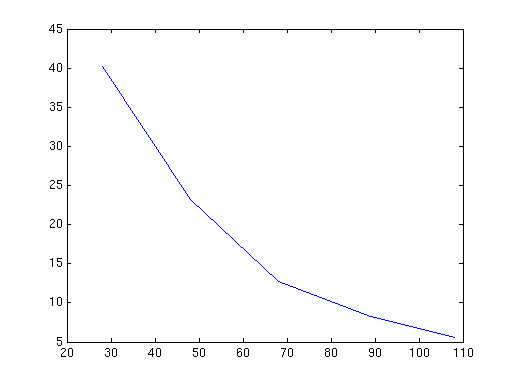
\includegraphics[width=50cm,height=26cm]{images/gmeans_k_vs_metric.png} 
         \column{.3\linewidth}
Here we plot the average Anderson-Darling statistic across all
clusters as a function of k. We can see how we arrive at a value of k
to use when the statistic crosses the threshold (6).
       \end{columns} 

       \noindent{\textbf{Davies-Bouldin Index}}\par Another way to
       determine k is via the DB Index.  It favors sets of clusters
       with high intra-cluster similarity and low inter-cluster
       similarity.  The formula is as follows:\newline

$X_j$ is sample $j$\\
$A_i$ is the center of cluster $i$\\
$T_i$ is the number of samples assigned to cluster $i$\newline

$S_i$ measures the intra cluster similarity of cluster $i$\\
$S_i = (\frac{1}{T_i} \sum\limits_{j=1}^{T_i} (X_j -
A_i)^q)^{\frac{1}{q}}$\newline

$M_{ij}$ measures the inter cluster similarity of clusters $i$ and $j$\\
$M_{ij} = (\sum\limits_{k=1}^{N} |a_{ki} - a{kj}|^p)^{\frac{1}{p}}$\newline

$DB$ is the Davies Bouldin index\\
$DB = \frac{1}{N} \sum\limits_{i=1}^N \max_{j:i \neq j} R_{ij}$\newline

The following is a graph of k vs DB:\newline

\begin{columns}[b]
  \column{.66\linewidth}
  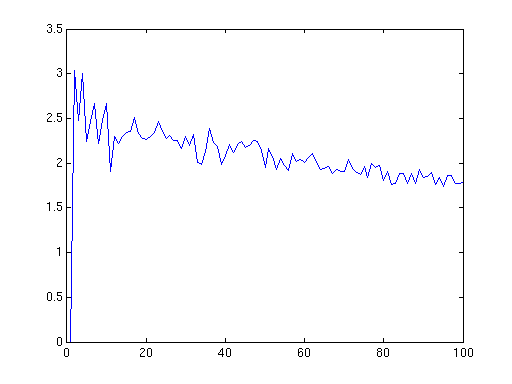
\includegraphics[width=60cm,height=36cm]{images/davies_k_vs_davies_index.png}
  \column{.2\linewidth}  
\end{columns} 



      \end{block}

       \begin{block}{Conclusion}
        \vskip1ex
        \noindent{\textbf{Conclusions}}
        \begin{itemize}
        \item Achieved result close to graph-structure based link predictors
        \item Experiments show that success of prediction comes from
          having \alert{accurate univariate link potential}
         \item Model preserves information
          \item \alert{Adding classifications of people does not significantly
          add to predictive power}
          \begin{itemize}
            \item May be because Email is poor indicator of useful
              class partitioning
            \end{itemize}
        \end{itemize}

        \vskip1ex
        \noindent{\textbf{Learnings}}
        \begin{itemize}
        \item Make sure features chosen have \alert{suffient
          mutual informtion} with variables of interest 
        \end{itemize}

        \vskip1ex
        \noindent{\textbf{Future Work}}
        \begin{itemize}
          \item Try with features of email that may be more indicitive
            of future communications
          \item Try in domain that has \alert{more direct features} of who a
            person may communicate with
            \begin{itemize}
              \item Facebook information would allow for application
                to social network structure as well as indicitive
                features of each person including location, school,
                interests, etc.
            \end{itemize}
          \item Test model in scenario where limited amounts of test
            data are observable
         \end{itemize}

        \vspace{-1ex}
      \end{block}
%%%%%%%%%%%%%%%%%%%%%%%%%%%%%%%%%%%%%%%%%%%%%%%%%%%%%%%

    \end{column}
  \end{columns}
\end{frame}

\end{document}


%%%%%%%%%%%%%%%%%%%%%%%%%%%%%%%%%%%%%%%%%%%%%%%%%%%%%%%%%%%%%%%%%%%%%%%%%%%%%%%%%%%%%%%%%%%%%%%%%%%%
%%% Local Variables: 
%%% mode: latex
%%% TeX-PDF-mode: t
%%% End: 
